\section{The Basic Structure of Particle Systems}
From an object-oriented programming point of view a \textbf{particle system} is a simple container object which manages all the \textbf{particles} inside it. At first the container is completely empty. The container then starts adding a constant or variable number of particles per frame to itself. This container has an interface which can be used by programmers to control the particles inside it and also some properties of the container itself. But how does one design and implement such a container?\\

Here are three short steps which can be carried out in order to obtain an object-oriented model of the problem:
\begin{enumerate}
	\item In order to highlight some of the base components of an object-oriented system write down a detailed description of the problem which the system is supposed to solve.
	
	\item Iterate through the description and identify all the nouns, adjectives and verbs. The nouns represent potential class names, the verbs represent potential class attributes and the verbs represent potential class methods.
	
	\item Assign attributes and methods to classes.
\end{enumerate}

Following is a description of a particle based graphical effect.

\newpage

Let us assume that we are asked to implement multiple particle effects using particle systems. Some particles may react to external forces in a different manner than others. For example some particles can be affected by gravity while others can not. Other particles can have a very high mass making their trajectory only slightly modifiable by an external wind force. Every particle should have a trajectory weather it is influenced by an external force or not.\\

Some particle systems may emit more than one type of particles. For example a particle system which simulates the explosion of a nuclear bomb should emit both lightweight and heavy particles. The heavy particles will fall down to the ground while the lightweight particles will form a cloud of fire, smoke and dust. The fire will burn out but the smoke and dust will get carried away by external wind forces if they exist.\\

A few basic components can be easily identified in the above problem description. This components are actually classes and they can be named as follows:

\begin{itemize}
	\item Particle
	\item FireParticle
	\item SmokeParticle
	\item DustParticle
	\item ParticleSystem
	\item FireSystem
	\item SmokeSystem
	\item DustSystem
\end{itemize}

No matter how high is the difference between a particle system and another one there will still be state and behavior which is common to all particle systems. The same statement is valid for the Particle classes as well. The Particle class should be a class which the other particle classes (FireParticle, SmokeParticle, etc...) can use to inherit common functionality from. The ParticleSystem class should be the class which holds the functionality common to all the particle system classes (FireSystem, SmokeSystem, etc...). But this is just a simple class structure which can be used to model particle systems. What is the actual mechanism which makes particle systems work? These steps are executed whenever most particle systems get rendered on a screen:

\begin{enumerate}
	\item New particles are created in order to be added to the particle system which is initially completely empty.
	\item All the attributes of the newly created particles are initialized.
	\item The list of particles contained by the particle systems is scanned for dead particles in order to remove them from the list.
	\item All the particles which still exist in the system will be moved to their new position. Each new position is computed with respect to the old position of the particle and attributes like direction, speed and acceleration.
	\item Finally an image of the particle system is rendered on the screen.
\end{enumerate}

Each step is described in a more detailed manner in the following subsections.

\newpage
\subsection{The Particle Spawning Step}
This is the first step in the rendering process of a particle system. This is when new particles are born. The number of particles generated per frame can contribute to the visual quality of a particle system. For example a real burning flame will not always have the same intensity meaning that it will not generate a constant number of fire particles. Using some kind of stochastic process to compute the number of particles generated per frame may make a simulated flame look more real, but for simplicity one can easily set the number of particles generated per frame to be constant.\\

One good example of a stochastic method which can be used to compute the number of particles generated per frame is to use a mean and a variance counter. The mean counter represents the average number of particles generated throughout a sequence of frames and the variance counter represents the largest possible difference between the average and the actual number of particles generated per one frame. The following formula shows exactly how this is supposed to work:
\begin{center}
	$n = m + r \cdot v$,
\end{center}
where $n$ is the number of particles generated per frame, $m$ is the mean, $v$ is the variance and $r$ is a random number between $-1$ and $1$.\\

Depending on the number of particles generated per frame, the memory consumption of particle systems can be quite high. Fortunately there is a method which can sometimes reduce their memory consumption. This method requires the inclusion of the screen area covered by the particle system in the equation. In other words if a particle system is very far away from the camera then it will appear to be very small thus a smaller number of particles will not affect the quality of the rendered image. There is no need to use $100,000$ particles to render a particle system which takes only 1 to 2 squared centimeters of the screen. The formula looks as follows:
\begin{center}
	$n = (m + r \cdot v) \cdot s$,
\end{center}
where $n$ is the number of particles generated, $m$ is the average number of particles generated over a period of time, $v$ is the variance, $r$ is a random number between $-1$ and $1$ and $s$ represents the screen area covered by the particle system.\\

\newpage
\subsection{The Particle Initialization Step}
While from a physics point of view a particle can be anything from a photon to a few water molecules or a even star, from an object oriented programming point of view a particle is a simple object which has a state and a behavior. The attributes of a particle represent its state and the methods of that particle represent a way to control its state. In this step all the particle attributes are initialized. Particles can have a very wide variety of different attributes but the most basic ones are listed bellow.
\begin{itemize}
	\item position
	\item speed
	\item acceleration
	\item size
	\item color
	\item lifetime
	\item texture
\end{itemize}

The position attribute should be implemented as a two-dimensional or a three-dimensional vector variable depending on the coordinate system. This variable is usually initialized with the origin of the particle system. In order to move a particle to a new position one would have to execute various mathematical vector operations on this variable. \\

The speed attribute should also be implemented as a vector and it should be used together with the acceleration attribute in order to modify a particle's position. This formula shows how to do this:
\begin{center}
	$\vec{n} = \vec{o} + (\vec{s} + \vec{a}),$
\end{center}
where $\vec{n}$ is the new position vector, $\vec{o}$ is the old position vector, $\vec{s}$ is the speed vector and $\vec{a}$ is the acceleration vector. The magnitude of the speed vector can remain constant throughout the whole lifetime of a particle while the magnitude of its acceleration vector can get random values from a predefined range in order to give the particle a more complex movement.\\

From a conceptual point of view a particle is a simple point in space. The downside to implementing particles as points is that points can not be textured. This is why particles are usually implemented with billboards. Billboards offer the possibility of obtaining textured particle effects. In the case of a square billboard the size attribute is actually the distance between the center of the billboard and one of its edges whereas in the case of a point implementation the size attribute represents the surface area covered by the point on the screen.\\

The color attribute can be used to control the color tone of a particle. In other words even if a particle has a texture with blue accents by changing this attribute one can make its texture to have reddish accents.\\

The lifetime attribute is used to decide when a particle is dead and needs to be removed from the particle system but this attribute can also be used to control a particle's opacity. A particle's opacity usually has values between $0.0$ and $1.0$. When a particle's opacity is at it's lowest bound the particle is completely transparent and when its opacity is at its highest bound the particle is completely opaque. If we make the particle's lifetime start with $1.0$ and decrease at each frame with a constant or variable amount we can control both the duration and the transparency of a particle with a single variable.\\

The texture attribute controls the texture of a particle and it can be implemented with a single texture variable or with a texture array variable. When it is implemented with an array a particle instance will be more dynamic because it will have multiple different textures throughout its lifetime.\\

\newpage
\subsection{The Dead Particle Removal Step}
In this step the list of particles managed by the particle system is scanned for dead particles. Whenever a dead particle is found it is quickly removed from the system. The scanning can be done starting from the beginning of the list or from the end.\\

When the scan is done starting from the beginning of the list a small glitch occurs at each pass. Whenever a particle is removed from the list, all the following particles in the list are moved to left with one position, this causes the pass to skip the verification of one particle. The skipped particle will be verified at the next pass but not having a particle removed when it is expected for it to be removed is not what we want.\\

In order to avoid this glitch one should iterate through the list starting from the end of the list. This way when a particle is removed the subsequent particles are moved in front of the verification index not in the back of it.\\

There may be times when we are unable to iterate backwards through a list. This is where \textbf{Iterator}s come in handy. Most programming languages (Java is one of these languages) offer these objects. When one uses an Iterator to scan a list of objects he does not need to worry about glitches like skipping an object because this matter is handled by the Iterator itself.\\

What are the conditions which need to be satisfied by a particle in order for it to be dead? One method of determining this is to keep track of a lifetime value which is supposed to drop with each rendered frame.\\

The distance between a particle's current position and the origin of the particle system can also be used to determine when a particle leaves a certain region surrounding the origin of the system. If that distance exceeds a certain value, the particle will be removed from the particle system.\\

\newpage
\subsection{The Particle Update Step}
In this step all the particles from a particle system are updated. Usually a particle update means moving it to a new position in space. But other particle attributes can also be affected by the update. Making the update affect other attributes will make the particle more dynamic.\\

The texture attribute is one of the attributes which can be updated. When it comes to texturing a particle one can use a single texture or a texture atlas (a whole range of textures). The texture update may mean to change the current texture with a new texture from the texture atlas. Thus giving a fire particle effect a more realistic look because in real life fire particles have variable shapes and sizes.\\

Let us assume that one wants to implement a particle effect that resembles a rainbow. This means that a particle from that particular particle system must morph through all the colors of the rainbow. This change of color can and should be done here in the update step.\\

Another particle attribute that can be updated is the size of the particle. Updating the size of a particle means to make it grow or shrink throughout its lifetime. So a particle may start really small at the origin of the particle system and become really large by the time it dies or vice versa.

\newpage
\subsection{The Particle Display Step}
A particle can be implemented in more than one way. For example the particles which formed the Genesis Effect from Star Trek II: The Wrath of Khan were implemented with light sources. The light sources combined themselves with each other in an additive manner regarding their color and transparency values. This technique had the advantage of removing the hidden surface problem because the particles did not obscure each other but simply added more light to a certain pixel.\\

A second method would be to use billboards to represent particles. A simple rectangle made out of two simple triangles can be a billboard. In fact any two-dimensional element rendered in a there-dimensional environment can be a billboard. The main difference between billboards and simple triangles is that a billboard always rotates itself around one or more axes in order to face the camera. There are advantages and disadvantages to using billboards instead of light sources.\\

One advantage is that billboards can be textured with more than one texture over their lifetime. A disadvantage is that billboards may need to be decreasingly sorted according to their distance from the camera. In other words the billboards which are further from the camera need to be rendered before the billboards which are closer to the camera otherwise the blending effect will be spoiled.\\

\newpage
\section{Billboards}
Particles can be displayed as simple colored points or as fully textured billboards. The obvious advantage of billboards is that they can be textured offering programmers the possibility to implement a very wide variety of textured particle based graphical effects.\\

A billboard is usually implemented with a quad made out of two triangles welded together because graphic cards render triangles faster. So a particle can be a simple textured quad. Only there is a problem with plain old quads.\\

Let us assume that a graphics programmer implements a graphic application which relies on particle systems and offers its users the possibility to change the camera position at will. If our programmer uses simple quads to render the particles the user can move the camera to positions from where he would only see a part of a specific particle or no particles at all (this can happen only when the back-face culling option is enabled and the camera is placed exactly in the back of the particles).\\

Imagine that we would like to see the particle effects from any position possible so having them visible only from some positions is unacceptable. We could disable the back-face culling option but then we would encounter other problems.\\

Firstly we would have to texture all particles on both sides which, besides the performance downsides, can be a little difficult. The performance downsides of this approach are memory consumption and more calls to the underlying graphics API.\\

And secondly there will still be positions from where the user will not be able to see the particles correctly. A particle watched from the sides will look like a vertical line. This might not be the desired result for most of us so this approach is a no-go. However there is an advantage to this approach, one can use two different textures for each of the sides of the particle. This might be useful at some point.\\

The simplest solution to this problem is to make the quads rotate in such a manner that they will always face the camera. This rotation is what differentiates a billboard from a simple quad and fortunately, there are a few techniques which can be used to achieve it.\\

\newpage
When it comes to billboard rotations the most basic and most used are the cylindrical and the spherical rotations. One can invent other different billboard rotation types according to his or her needs but the two basic rotation types solve most of the problems related to billboards.\\

The rotations of a billboard can be towards any object or point in the scene not just towards the camera. However rotating a billboard towards a certain point is not the only option. There is a technique which can be used to fake true billboarding.\\

Let us take the simple case when a billboard has to rotate itself towards the camera. Instead of making it rotate exactly towards the point where the camera lies we can make it rotate towards a plane perpendicular to the cameras looking direction vector. This technique is sometimes called fake billboarding because it is an approximation of what a true billboard does. Tough it is just an approximation it might be perfect for some applications and sometimes easier to implement.\\

The two basic billboard rotation mechanisms (the cylindrical and spherical rotation types) do true billboarding, meaning that both mechanisms make the quad rotate itself exactly towards the point where the camera lies.

\newpage
\subsection{The Cylindrical Rotation Mechanism}
When using this mechanism the rotation of the billboard is restricted by one axis. Figure 2.1 shows a billboard composed from two triangles. The red vertical line which intersects it represents its rotation axis.

\begin{figure}[h]
	\caption{Rotation axis of a billboard}
	\centering
	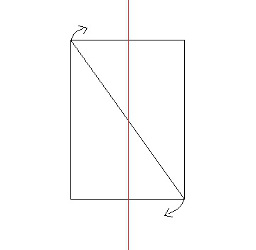
\includegraphics{billboard_axis.jpg}
\end{figure}

Notice that the billboard is a vertical slice of a cylinder. The slice goes exactly through the central axis of the cylinder. Actually the rotation axis of the billboard and the axis of the cylinder are one and the same.\\

If we would rotate the billboard from Figure 2.1 fast enough it would appear to look exactly like a cylinder. This is why the billboards which are implemented with this techniques are sometimes referred to as cylindric billboards.\\

\newpage
\subsection{How To Implement Particles as Quads}
Implementing a particle as a simple quad is fairly easy. Let us start with the center of the particle. This point is supposed to be used to control the movement of the particle. When one changes the coordinates of this point the coordinates of the corners of the particle will also change. This is because the values of the corner coordinates depend on the value of the particle center coordinates.\\

With these coordinates one can compute the corner coordinates of the particle but he can also move the particle by changing this coordinate.\\


\newpage
\subsection{Other Applicabilities of Billboards}
Although billboards are useful for implementing textured particle systems they can also be used to reduce the triangle count of other three-dimensional objects.\\

Let us take as an example a tree. If a programmer were to render a tree using triangles he would have to face a trade-off between detail and rendering speed. In other words if he would use a small number of triangles the rendering speed will be high but the detail level of the tree will be fairly low thus making the tree look unrealistic.\\

On the other hand if our programmer were to use a very high triangle count the detail level of the tree will be high but the rendering speed would be lower. Actually the difference will not be that noticeable when rendering a single tree but when one renders a whole forest the difference will be greater.\\

Fortunately we have modern hardware which can handle rendering scenes with a high polygon count very well. But for the times when we do not have modern hardware or we simply want to optimize the rendering speed of a graphic application for no reason we have \textbf{billboards}.\\

Billboards can be easily used to render a forest. In the rendering process of the forest we can use a billboard (one made out of two triangles not a few thousands) for each tree in the forest. This will increase the rendering speed of the graphic application without loosing that much on the detail side of the application.\\

Billboards are perfect for the task of reducing the polygon count of graphic applications because a tree can be represented with only two triangles and they do not break the tree illusion because they always rotate their face towards the camera.\\